\section{Red de Oficina}

Para este experimento se tomo una captura de 20 minutos de la red Wi-Fi de una oficina, sin conocimientos
previos de esta.

\subsection{Fuente binaria S}

\begin{figure}[H]
  \centering
    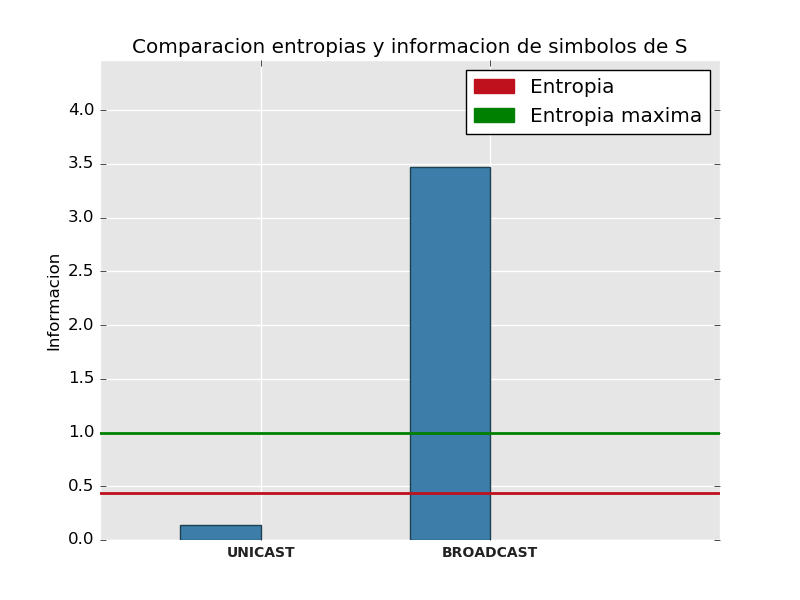
\includegraphics[width=0.45\textwidth]{agutter/gr1.png}
  \caption{Entropia de la fuente S}
  \label{entropia-s-agutter}
\end{figure}

Como podemos ver en el gráfico, y al igual que en casos anteriores, la entropía dista de ser máxima.
De hecho, es claro que el símbolo $BROADCAST$ proporciona considerablemente m\'as información que el
$UNICAST$. 

Podemos entonces deducir que la red cuenta con un mayor flujo de paquetes Ethernet $UNICAST$ que
$BROADCAST$, lo que podría atribuirse a regulares cambios en la topología de la red.

Esto se corresponde a el comportamiento esperado, dado que se trata de una red Wi-fi abierta a la que
probablemente distintos dispositivos se conecten y desconecten con frecuencia, afectando as\'i, la
topolog\'ia de la misma.

\begin{table}[H]\begin{center} %ht
  \begin{tabular}{|c|c|}
    \hline
    \textbf{Nodo} & \textbf{Información} \\ \hline
    \texttt{UNICAST}& 0.136783 \\ \hline
    \texttt{BROADCAST}& 3.466655 \\ \hline
  \end{tabular}
  \caption{Información de los símbolos de S}
  \label{info-simbolos-agutter}
\end{center}\end{table}

Podemos imaginar que el overhead impuesto por la red influencia la entropía de esta fuente, ya que
en caso de tener un menor overhead, la informaci'on del s\'imbolo $S_{BROADCAST}$ se reducir\'ia y
la entrop\'ia de la fuente $S$ aumentar\'ia, acerc\'andola al m\'aximo.

\subsection{Red de Mensajes ARP subyacente}

\begin{figure}[H]
  \centering
    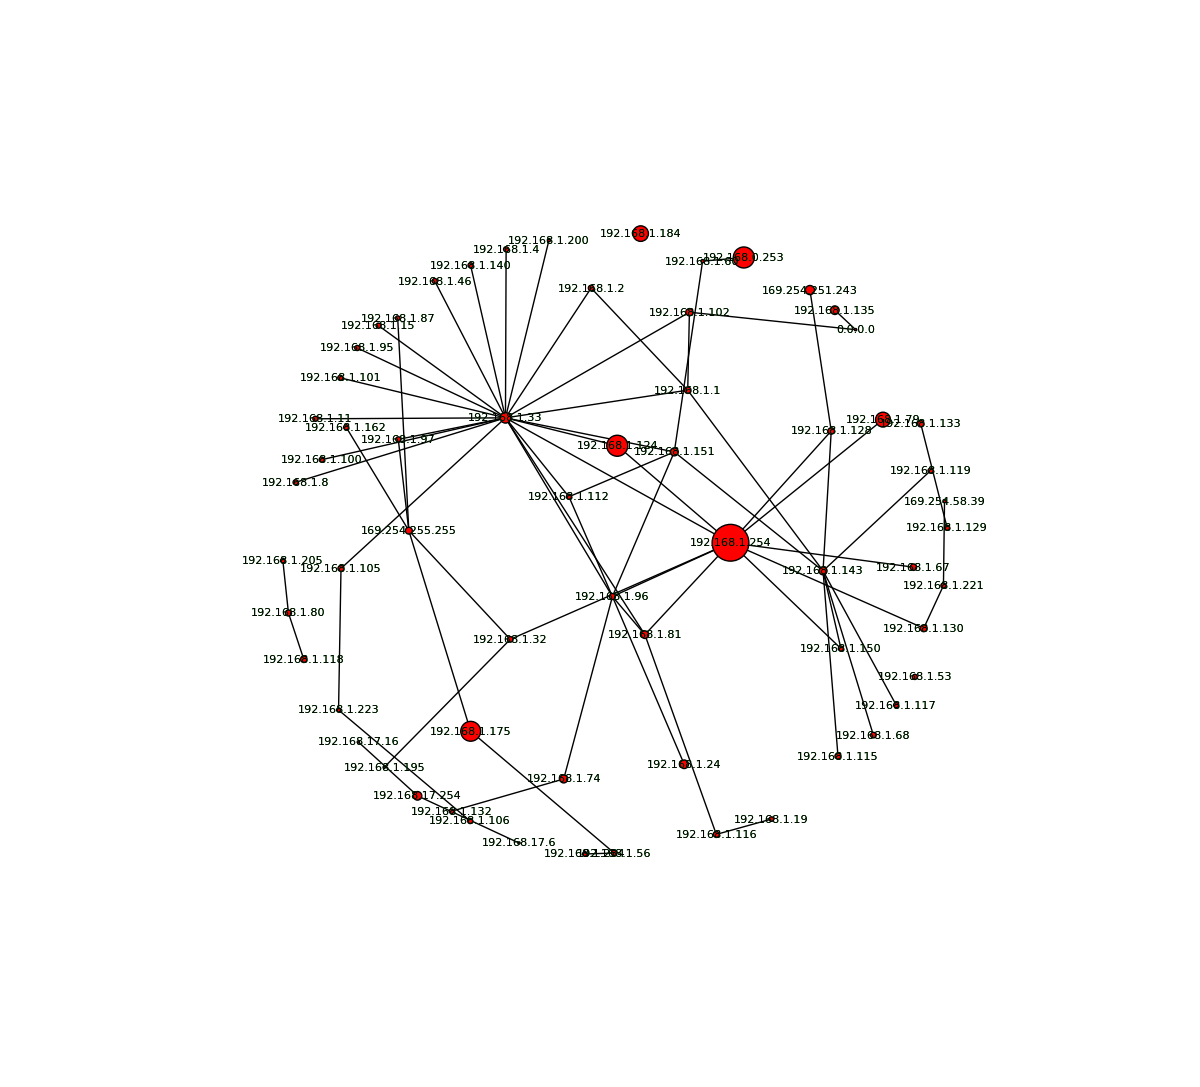
\includegraphics[width=0.45\textwidth]{agutter/gr3.png}
  \caption{Red de Mensajes ARP subyacente}
  \label{grafo-s1-agutter}
\end{figure}

Analizando la cantidad de apariciones (tama\~no) de cada nodo en las tramas ARP y la distribuci\'on de
los v\'ertices, podemos ver que se trata de una red con alto tr\'afico pero mal distribuido:
la gran mayor\'ia de los nodos tiene poca comunicaci\'on. Sin embargo, podemos f\'acilmente distinguir
a 192.168.1.254 como un nodo importante, seguido de 192.168.1.33, 192.168.1.124, 192.168.1.253 y
192.168.1.175.

Dado el tama\~no del nodo 192.168.1.254 y la cantidad de v\'ertices que alcanzan al nodo 192.168.1.33,
podr\'iamos intuir que se trata de posibles gateways de la red, ya que ejercen como centros de gravedad
del grafo, y se comunican con un gran n\'umero de nodos.

Adem\'as, podr\'iamos pensar que el nodo 192.168.1.124 corresponde a la salida de la red ya que tiene
un alto grado de impacto pero solo se comunica con los dos nodos anteriores.


\subsection{Fuente S1}

A continuaci\'on presentamos un gr\'afico comparando la cantidad de informaci\'on de cada s\'imbolo
con la entrop\'ia de la fuente, y una tabla presentando los nodos distinguidos detectados por la
herramienta.

\begin{figure}[H]
  \centering
    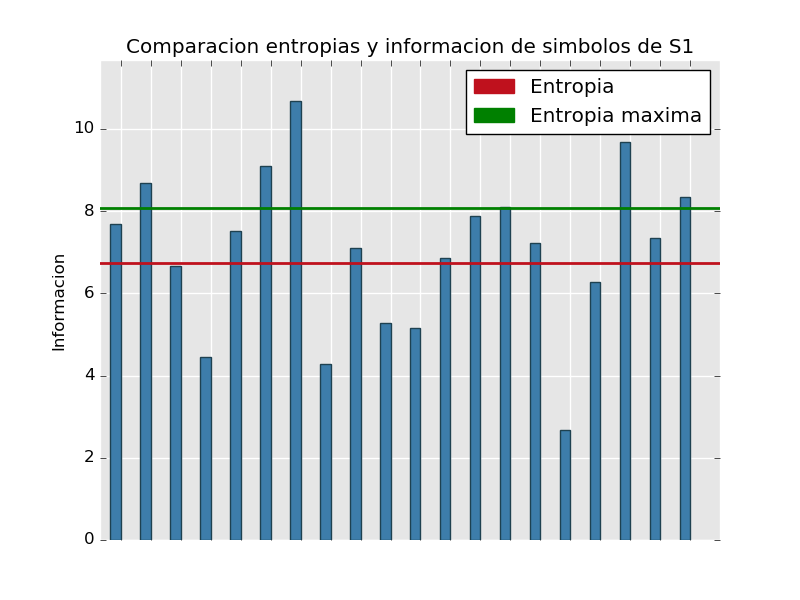
\includegraphics[width=0.45\textwidth]{agutter/gr2.png}
  \caption{Entropia de la fuente S1}
  \label{entropia-s1-agutter}
\end{figure}

\begin{table}[H]\begin{center} %H
  \begin{tabular}{|c|c|}
    \hline
    \textbf{Nodo} & \textbf{Informacion} \\ \hline
    \texttt{192.168.1.254}& 2.672976 \\ \hline
    \texttt{192.168.1.253}& 4.286283 \\ \hline
    \texttt{192.168.1.124}& 4.286283 \\ \hline
    \texttt{192.168.1.175}& 4.449781 \\ \hline
    \texttt{192.168.1.184}& 5.155038 \\ \hline
    \texttt{192.168.1.79}& 5.286283 \\ \hline
    \texttt{192.168.1.33}& 6.286283 \\ \hline
    \texttt{192.254.251.243}& 6.678600 \\ \hline
  \end{tabular}
  \caption{Nodos distinguidos detectados por la herramienta}
  \label{Nodos-distinguidos-agutter}
\end{center}\end{table}

R\'apidamente podemos destacar que los nodos que distinguimos en el punto anterior son tambi\'en detectados
por la herramienta. Esto nos lleva a pensar que detectamos correctamente los posibles gateways de la red.

Observando el gr\'afico, podemos adem\'as ver que son pocos los s\'imbolos con informaci\'on menor a la
entrop\'ia de la fuente, y parecieran corresponderse a los detectados.

Podr\'iamos entonces concluir que el criterio de distinci\'on propuesto es bastante preciso, y quiz\'as
un an\'alisis m\'as fino permitir\'ia encontrar un\'ivocamente los gateways de la red.
